\documentclass[12pt]{article}
\usepackage[utf8]{inputenc}
\usepackage{amsmath}
\usepackage{amssymb}
\usepackage{graphicx}
\graphicspath{ {./plots/} }

\newcommand{\rectres}[1]{
\begin{center}
\begin{tabular}{ |c| }
\hline
 #1\\
\hline
\end{tabular}
\end{center}
}

\newcommand{\qed}{\hfill$\blacksquare$}

\title{Introduction to Numerical Optimization\\Assignment 1}
\author{Yair Nahum 034462796\\and\\Gadiel  }

\begin{document}

\maketitle

%\tableofcontents{}

\section{Analytical and Numerical Differentiation}

\subsection{Analytical Differentiation}

\subsubsection{Gradient and Hessian of $f_1$}
$$f_1(x)=\phi(Ax)$$
Where:
$$f_1:\mathbb{R}^n \rightarrow \mathbb{R}$$
$$x \in \mathbb{R}^{n},$$
$$A \in \mathbb{R}^{m\times n},$$
$$\phi:\mathbb{R}^m \rightarrow \mathbb{R}$$
Assuming $\nabla\phi$ and $\nabla^2\phi$ are known (relative to its $\mathbb{R}^m$ variable).
$$\nabla f_1 = ?$$
$$\nabla^2 f_1 = ?$$

We denote $u=Ax \Rightarrow du=Adx$, by the external definition of the gradient:
$$df_1=d\phi(u)=(\nabla\phi(u))^T du = (\nabla\phi(Ax))^T A dx = $$
$$ \langle A^T\nabla \phi(Ax), dx \rangle \Rightarrow $$
\rectres{$\nabla f_1 = A^T\nabla \phi(Ax)$}
Next, We denote $\nabla f_1= g(x)$:
$$dg\equiv Hdx,d(\nabla \phi(u)) =  \nabla^2 \phi(u) du \Rightarrow$$
$$dg=d(\nabla f_1) = d(A^T\nabla \phi(Ax))=A^Td(\nabla \phi(u))=A^T\nabla^2 \phi(u) du = A^T\nabla^2 \phi(Ax) A dx \Rightarrow$$
\rectres{$\nabla^2 f_1 = A^T\nabla^2 \phi(Ax) A$}

\subsubsection{Gradient and Hessian of $f_2$}
$$f_2(x)=h(\phi(x))$$
Where:
$$f_2:\mathbb{R}^n \rightarrow \mathbb{R}$$
$$x \in \mathbb{R}^{n},$$
$$\phi:\mathbb{R}^n \rightarrow \mathbb{R}$$
$$h:\mathbb{R} \rightarrow \mathbb{R},$$
Assuming $\nabla\phi, \nabla^2\phi, h'(t)$ and $h''(t)$ are known.
$$\nabla f_2 = ?$$
$$\nabla^2 f_2 = ?$$
We denote $t=\phi(x)\Rightarrow dt=d\phi(x)=(\nabla \phi(x))^Tdx$
$$df_2= dh = h'(t)dt = h'(\phi(x))(\nabla \phi(x))^Tdx=$$
Since $h'(t)$ is scalar, it doesn't change on transpose operation:
$$\langle h'(\phi(x))\nabla \phi(x), dx \rangle \Rightarrow$$
\rectres{$\nabla f_2 = h'(\phi(x))\nabla \phi(x)$}
Next, We denote $\nabla f_2= g(x)$:
$$dg = d(h'(\phi(x))\nabla \phi(x)) =  d(h'(\phi(x)))\nabla \phi(x) + h'(\phi(x))d(\nabla \phi(x))=$$
$$h''(\phi(x))((\nabla \phi(x))^Tdx)\nabla \phi(x) + h'(\phi(x))\nabla^2 \phi(x)dx=$$
$$h''(\phi(x))\nabla \phi(x)((\nabla \phi(x))^Tdx) + h'(\phi(x))\nabla^2 \phi(x)dx=$$
$$h''(\phi(x))\nabla \phi(x)(\nabla \phi(x))^Tdx + h'(\phi(x))\nabla^2 \phi(x)dx=$$
$$[h''(\phi(x))\nabla \phi(x)(\nabla \phi(x))^T + h'(\phi(x))\nabla^2 \phi(x)]dx=$$
by definition $dg=Hdx$, therefore:
\rectres{$\nabla^2 f_2 = h''(\phi(x))\nabla \phi(x)(\nabla \phi(x))^T + h'(\phi(x))\nabla^2 \phi(x)$}
\newpage
\subsubsection{Gradient and Hessian of $\phi$}
Given the following $\phi:\mathbb{R}^3\rightarrow\mathbb{R}$ function:
$$\phi \begin{pmatrix}x_1\\x_2\\x_3 \end{pmatrix} = cos(x_1x^2_2x_3)$$
We need to calculate its gradient vector and hessian matrix.
We can use the previous section results when there is a chain of functions to compute the gradient and hessian as we can define:
$$f=cos:\mathbb{R}\rightarrow\mathbb{R}$$ and $$u=x_1x^2_2x_3:\mathbb{R}^3\rightarrow\mathbb{R}$$
Thus, the gradient is as follows:
$$\nabla \phi = f'(u)\nabla u(x) = -sin(x_1x^2_2x_3)\begin{pmatrix}x^2_2x_3\\2x_1x_2x_3\\x_1x^2_2 \end{pmatrix}$$
\rectres{$\nabla \phi = -sin(x_1x^2_2x_3)\begin{pmatrix}x^2_2x_3\\2x_1x_2x_3\\x_1x^2_2 \end{pmatrix}$}\\
We can also use the hessian formula we got on the previous section and get:
$$\nabla^2 \phi = f''(u(x))\nabla u(x)(\nabla u(x))^T + f'(u(x))\nabla^2 u(x)=$$
$$-cos(x_1x^2_2x_3)\begin{pmatrix}x^2_2x_3\\2x_1x_2x_3\\x_1x^2_2 \end{pmatrix}\begin{pmatrix}x^2_2x_3 & 2x_1x_2x_3 & x_1x^2_2 \end{pmatrix} - sin(x_1x^2_2x_3)\begin{pmatrix}0 & 2x_2x_3 & x^2_2\\2x_2x_3 & 2x_1x_3 & 2x_1x_2\\x^2_2 & 2x_1x_2 & 0 \end{pmatrix} \Rightarrow$$
\rectres{$\nabla^2 \phi = -cos(x_1x^2_2x_3)\begin{pmatrix}x^4_2x^2_3 & 2x_1x^3_2x^2_3 & x_1x^4_2x_3\\2x_1x^3_2x^2_3 & 4x^2_1x^2_2x^2_3 & 2x^2_1x^3_2x_3\\x_1x^4_2x_3 & 2x^2_1x^3_2x_3 & x^2_1x^4_2 \end{pmatrix} - sin(x_1x^2_2x_3)\begin{pmatrix}0 & 2x_2x_3 & x^2_2\\2x_2x_3 & 2x_1x_3 & 2x_1x_2\\x^2_2 & 2x_1x_2 & 0 \end{pmatrix}$}

\subsubsection{First and Second Derivatives of $h$}
$$h=\sqrt{(1+sin^2(x)}$$
We can solve directly using derivative formulas and we can use the external gradient definition.\\
We can denote $v(x)=sin(x),u(v)=1+v^2$ and $h = f(u)=\sqrt{u} \Rightarrow$ 
$$h=f(u(v)) \Rightarrow$$
$$dv=d(sin(x))=cos(x)dx$$
$$ du=2vdv$$
$$ dh=df(u)=\frac{1}{2}\frac{1}{\sqrt{u}}du$$
$$\Rightarrow$$
$$dh=\frac{1}{2}\frac{1}{\sqrt{u}}du=\frac{1}{2}\frac{1}{\sqrt{1+v^2}}2vdv=\frac{sin(x)cos(x)}{\sqrt{1+sin^2(x)}}dx \Rightarrow$$\\
\rectres{$h'(x)=\frac{sin(x)cos(x)}{\sqrt{1+sin^2(x)}}$}
For the second derivative we can define the following functions and compute again using total derivative rules:\\
$$v(x)=sin(x)$$ 
$$t(x)=cos(x)$$
$$u(v)=1+v^2$$
$$z(u)=\sqrt{u}$$
$$q(z)=\frac{1}{z}$$
$$h' = f(q,v,t)=vtq\Rightarrow$$
$$dv=cos(x)dx$$
$$dt=-sin(x)dx$$
$$du=2vdv$$
$$dz=\frac{1}{2\sqrt{u}}du$$
$$dq=-\frac{1}{z^2}dz$$
We also know according to total differential:\\
$$dh'=d(f(v,t,q))=d(vtq)=qtdv+qvdt+vtdq$$
We put the previous differentials and get:\\
$$dh'=qtdv+qvdt+vtdq=\frac{tdv+vdt}{z}-\frac{vt}{z^2}dz=\frac{tdv+vdt}{\sqrt{u}}-\frac{vt}{u}\frac{1}{2\sqrt{u}}du=$$
$$\frac{tdv+vdt}{\sqrt{1+v^2}}-\frac{vt}{2(1+v^2)\sqrt{1+v^2}}2vdv=\frac{cos^2(x)-sin^2(x)}{\sqrt{1+sin^2(x)}}dx-\frac{sin^2(x)cos^2(x)}{(1+sin^2(x))^{\frac{3}{2}}}dx$$
$$\Rightarrow$$
\rectres{$h''(x)=\frac{cos^2(x)-sin^2(x)}{\sqrt{1+sin^2(x)}}-\frac{sin^2(x)cos^2(x)}{(1+sin^2(x))^{\frac{3}{2}}}$}

\subsubsection{Analytical Evaluation}
in code

\subsection{Numerical Differentiation}
\subsubsection{Numerical Gradient}
Background information given in the assignment's pdf
\subsubsection{Numerical Hessian}
Background information given in the assignment's pdf
\subsubsection{Numerical Evaluation of Gradient and Hessian}
in code

\newpage

\subsection{Comparison}
See hw1.py for the code that does the comparison.
With random seed set to 10 we got the following results:\\
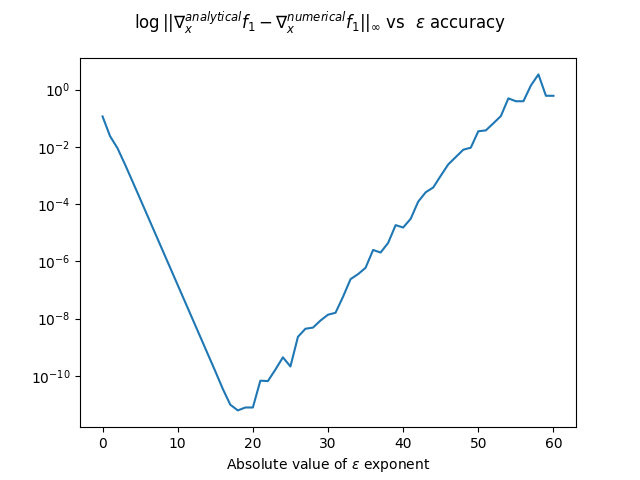
\includegraphics[scale=0.7]{f1_grad_plot}\\
f1 gradient min infinity norm error : 6.255884699157832e-12\\
epsilon exponent: -18\\
epsilon value: 3.814697265625e-06\\
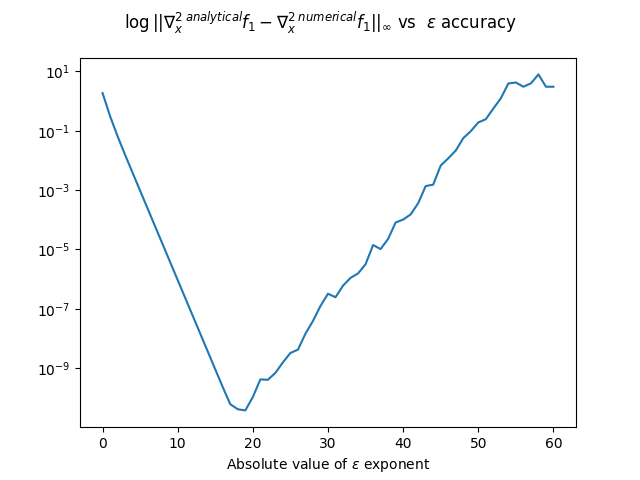
\includegraphics[scale=0.7]{f1_hessian_plot}\\
f1 hessian min infinity norm error : 3.76653153111306e-11\\
epsilon exponent: -19\\
epsilon value: 1.9073486328125e-06\\
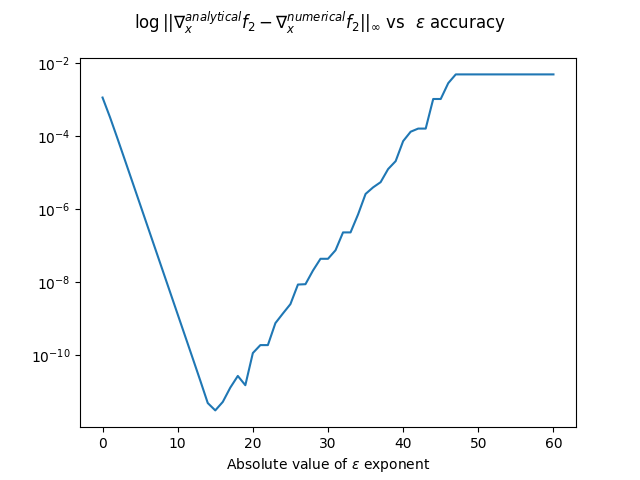
\includegraphics[scale=0.7]{f2_grad_plot}\\
f2 gradient min infinity norm error : 3.0824258076544986e-12\\
epsilon exponent: -15\\
epsilon value: 3.0517578125e-05\\
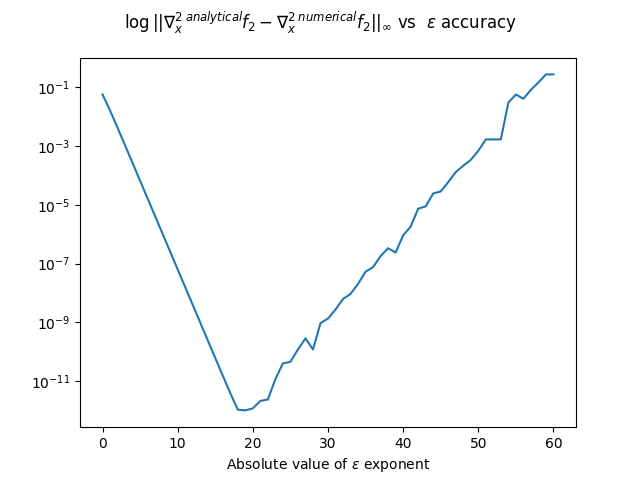
\includegraphics[scale=0.7]{f2_hessian_plot}\\
f2 hessian min infinity norm error : 1.0314180065584821e-12\\
epsilon exponent: -19\\
epsilon value: 1.9073486328125e-06\\

\newpage
\section{SVD}
\subsection{Motivation}
Background information given in the assignment's pdf
\subsection{Singular Value Gradient}
We need to calculate the gradient of $f_i(A) = \sigma_i$\\
Given SVD of $A$ as $$A=USV^T$$
In which $U$ and $V$ are orthonormal matrices:
$$U \in \mathbb{R}^{m\times m}$$
$$V \in \mathbb{R}^{n\times n}$$
And S is a rectangular diagonal matrix with:
\[
    S_{i,j}= 
\begin{cases}
    \sigma_i,& \text{if } i==j\\
    0,       & \text{otherwise}
\end{cases}
\]
We will try to define the function $f_i(A)$ based on its SVD decomposition and apply the external definition of the gradient.\\
\subsubsection*{Lemma1}
$$A=USV^T=\sum_{k=1}^p\sigma_k u_{k} v^T_{k}$$ When $p=\min(m,n)$
\subsubsection*{Proof}
$$A_{i,j}=(USV^T)_{i,j}=\sum_{k=1}^n U_{i,k} (SV^T)_{k,j}=\sum_{k=1}^m U_{i,k} \sum_{l=1}^n S_{k,l}V^T_{l,j}=\sum_{k=1}^m \sum_{l=1}^n U_{i,k}  S_{k,l}V^T_{l,j}$$
Since S is a rectangular diagonal matrix we actually have only one summation up to $p=\min(m,n) \Rightarrow$:
$$\sum_{k=1}^m \sum_{l=1}^n U_{i,k}  S_{k,l}V^T_{l,j}=\sum_{k=1}^p U_{i,k}  S_{k,k}V^T_{k,j} =\sum_{k=1}^p\sigma_k U_{i,k}V^T_{k,j} \Rightarrow$$
$$(*)\:\:\:\:A_{i,j}=\sum_{k=1}^p\sigma_k U_{i,k}V^T_{k,j}$$
On the other hand, if we denote the column vectors of $U$ as $u_k$ and the row vectors of $V^T$ as $v^T_k$,
due to linearity of matrices addition, we can deduce:
$$\Big(\sum_{k=1}^p\sigma_k u_{k} v^T_{k}\Big)_{i,j}=\sum_{k=1}^p\sigma_k \Big(u_{k} v^T_{k}\Big)_{i,j}$$
In addition, the following is also true (outer product):
$$\Big(u_{k} v^T_{k}\Big)_{i,j}=U_{i,k}V^T_{k,j}$$
So,
$$\Big(\sum_{k=1}^p\sigma_k u_{k} v^T_{k}\Big)_{i,j}=\sum_{k=1}^p\sigma_k \Big(u_{k} v^T_{k}\Big)_{i,j}=\sum_{k=1}^p\sigma_k U_{i,k}V^T_{k,j}\Rightarrow$$
$$(**)\:\:\:\:\Big(\sum_{k=1}^p\sigma_k u_{k} v^T_{k}\Big)_{i,j}=\sum_{k=1}^p\sigma_k U_{i,k}V^T_{k,j}$$
From $(*)$ and $(**)$ we get:
$$A_{i,j}=\Big(\sum_{k=1}^p\sigma_k u_{k} v^T_{k}\Big)_{i,j}$$
\qed\\
Another simpler way to look at it and prove the identity, is to notice (linear algebra fact) that any matrix multiplication can be constructed using outer products of columns and rows:
$$C \in \mathbb{R}^{m\times p}$$
$$D \in \mathbb{R}^{p\times n}$$
$$CD=\sum_{k=1}^p c_{k} d^T_{k}$$
Thus,
if we define $C=US, D=V^T$, we get that the vectors are actually:  
$$c_{k}=\sigma_k u_{k}, d_{k}=v_{k}$$
When:
$$p=\min(m,n), k \in [1..p]$$
$$c_{k} \in \mathbb{R}^{m}$$
$$d_{k} \in \mathbb{R}^{n}$$
And the identity is then driven straight forward.
\qed\\
\subsubsection*{Lemma2}
$$f_i(A)=\sigma_i=u_i^T A v_i$$
\subsubsection*{Proof}
From previous Lemma and orthonaormality of the $U,V$ matrices:
$$u_i^T A v_i=u_i^T \Big(\sum_{k=1}^p \sigma_k u_{k} v^T_{k}\Big)v_i=\sum_{k=1}^p \sigma_k u_i^T  u_{k} v^T_{k}v_i = \sum_{k=1}^p \sigma_k \delta_{i,k}=\sigma_i$$
\qed\\
Now, we can find the gradient using the external definition of the gradient and the trace properties:
$$d(f_i(A))=d(\sigma_i)=d(\sigma_i)=d(trace(\sigma_i))=d(trace(u_i^T A v_i))=d(trace(v_i u_i^T A )) = $$
$$trace(d(v_i u_i^T A ))=trace(v_i u_i^T dA ) = \langle u_i v_i^T, dA \rangle \Rightarrow$$
\rectres{$\nabla f_i(A)=u_i v_i^T$}
\end{document}

